\chapter{Evaluation of Performance}
\label{chapter:evaluation}

In this chapter, I evaluate the framework's performance by measuring the duration of analysing several source code repositories.


\section{Evaluation Environment}

\subsection{Computer Configuration}

The measurements were performed on my computer for the sake of simplicity. During a measurement session, my computer was plugged in, it was configured to utilise its full performance, and only those software were running, which were explicitly necessary for the measurements. Each measurement was preceded by a full system reboot.

The major points of the my computer's configuration is the following:

\begin{itemize}
\item Apple MacBook Pro, Mid-2014, 13 inches;
\item Intel Core i5, 2.6 GHz;
\item 8 GB 1600 MHz DDR3 RAM;
\item 250 GB SSD.
\end{itemize}


\subsection{Software Configuration}

As currently the Codemodel-Rifle framework does not have any interface to interact with, the measurements were performed as per-repository unit tests with logging test results onto the console.

\begin{itemize}
\item \textbf{Runtime:} JetBrains IntelliJ IDEA Ultimate 2016.3.4
\item \textbf{Java Runtime Environment:} 1.8.0\_112-release-408-b6 x86\_64
\item \textbf{Java Virtual Machine:} OpenJDK 64-Bit Server VM by JetBrains s.r.o (initial memory allocation pool: 4 GB, maximum memory allocation pool: 8 GB)
\item \textbf{Database:} Neo4j Community Edition 3.1.3 Server (initial heap size: 4 GB, maximum heap size: 8 GB, page cache size: 8 GB, transaction log retention policy: 1 day)
\item \textbf{Database driver:} Neo4j Bolt driver for Java 1.1.1
\end{itemize}

For better performance, a database index was defined in Neo4j for the \lstinline{`id'} property of all nodes labeled with \lstinline{'AsgNode'} (practically all nodes created by Codemodel-Rifle).


\section{Measurement Goals and Methods}

\subsection{Selection Criteria of the Analysed Source Code Repositories}

The evaluation was performed on popular open-source JavaScript code repositories found on GitHub. The 40 randomly chosen repositories differ in size, in the number of lines of code, and in the number of distinct source files. The repositories are listed in the Appendix.


\subsection{Key Performance Indices}

The goal of the performance evaluation was to determine the time characteristics of the refactored Codemodel-Rifle framework, and especially the implemented analyses. Based on the production operation of the framework detailed in the introduction of \Cref{chapter:elaboration}, the following four Key Performance Indices have been determined to be measured.

\begin{itemize}
\item \textbf{The duration of synchronisation:} the time period between starting the importing process of a code repository (excl. finding all \lstinline{.js} files, and reading the contents of the source files) and saving the last module's last \lstinline{AsgNode} into the database.
\item \textbf{The duration of interconnection:} this time period encompasses searching for semantically valid interconnections between modules, and actually performing the interconnections.
\item \textbf{The duration of running the Qualifier System:} this time period encompasses initialising the Qualifier System, and propagating the qualifiers.
\item \textbf{The duration of performing the analyses:} this time period encompasses trying to match all predefined analysis patterns.
\item \textbf{The total duration of the analysis process:} this time period is the sum of the above four durations. It was not measured, but calculated from the above.
\end{itemize}

Besides the Key Performance Indices, the number of nodes and relationships created during the synchronisation of a repository is also recorded.


\subsection{Process of Measurement}

All analysed code repositories were measured four times in a session in order to avoid biases caused by the environment. Each session was preceded by a full system restart. The final measurement results of a repository are averaged from the four different values.


\section{Measurement Results}

In this section, I present and evaluate the measurement results of the aforementioned Key Performance Indices.


\subsection{Synchronisation}

At first, the repository needs to be synchronised into Codemodel-Rifle. At this time, the source code files of the repository gets translated to distinct, per-module property graphs.

\begin{figure}[!htb]
	\centerfloat
	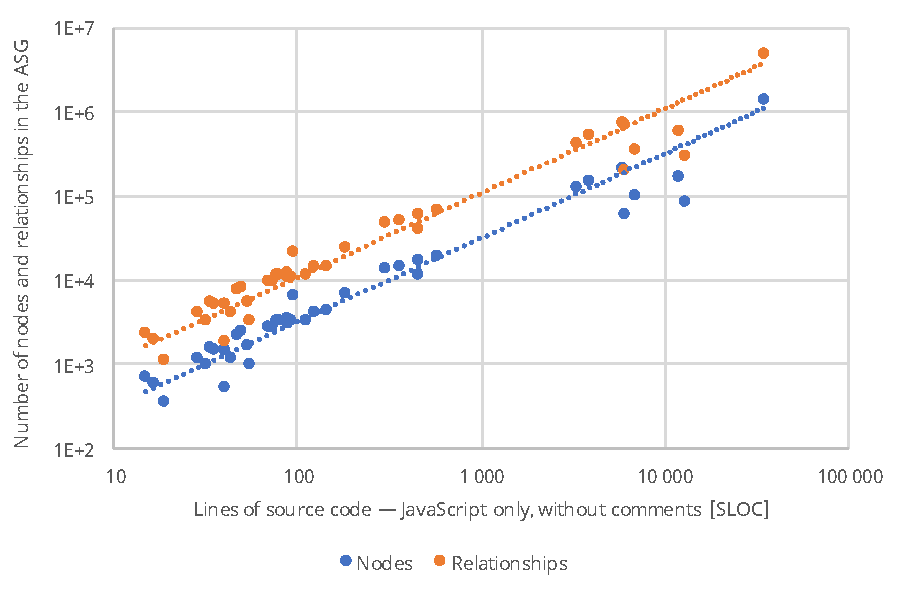
\includegraphics[width=\textwidth,clip]{figures/measurement-nodes-relationships-sloc.pdf}
	\caption{The characteristics of synchronising repositories into Codemodel-Rifle}
	\label{fig:measurement-nodes-relationships-sloc}
\end{figure}

There are many coding styles and conventions, and the contents of the source files can vary from per-line exported configuration constants to program codes without physical line breaks. Nevertheless, there is a linear relationship between the number of code lines and the number of created ASG nodes and relationships in the analysed repositories.

\Cref{fig:measurement-nodes-relationships-sloc} presents the correlation of the source lines of code (SLOC) and the number of ASG nodes and relationships created during synchronising the code bases into Codemodel-Rifle. In terms of SLOC, the smallest repository imported was \lstinline{initialstate/silent-doorbell} 15 lines of code (686 nodes and 2306 relationships created), while the largest was \lstinline{tresorit/webclient} with 34,546 lines of code (with 1,346,776 nodes and 4,576,319 relationships).


\begin{figure}[!htb]
	\centerfloat
	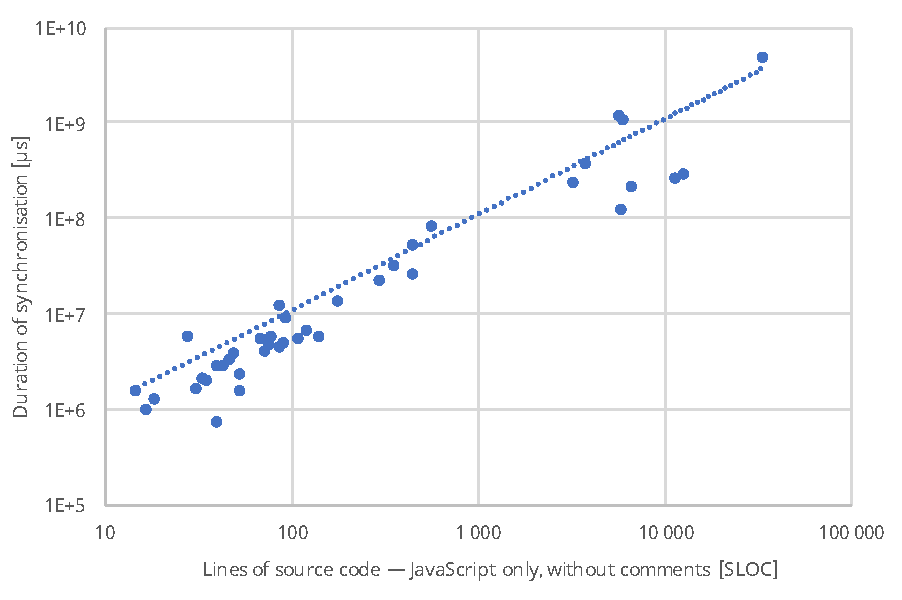
\includegraphics[width=\textwidth,clip]{figures/measurement-synctime-sloc.pdf}
	\caption{The characteristics of synchronising repositories into Codemodel-Rifle}
	\label{fig:measurement-synctime-sloc}
\end{figure}

\begin{figure}[!htb]
	\centerfloat
	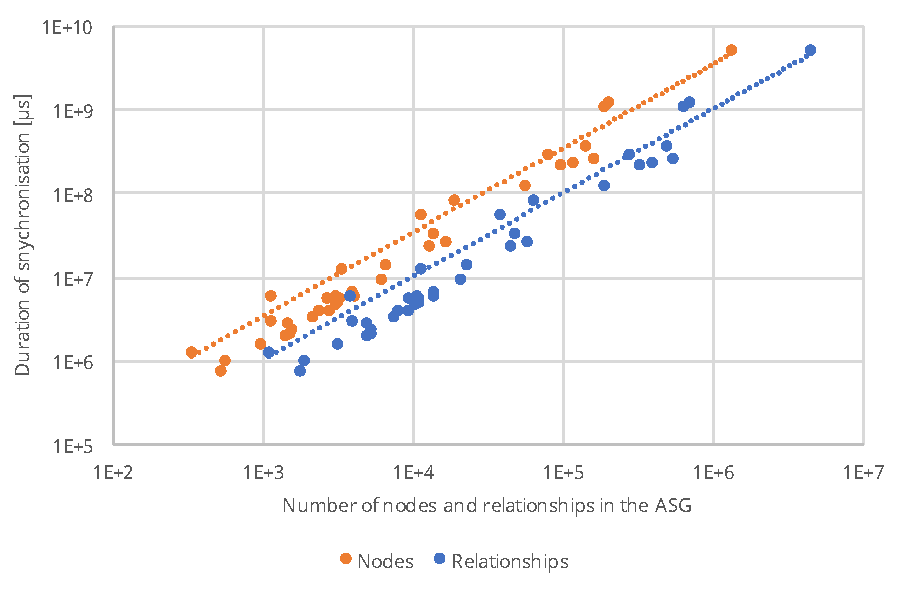
\includegraphics[width=\textwidth,clip]{figures/measurement-synctime-nodes-relationships.pdf}
	\caption{Synchronising repositories into Codemodel-Rifle}
	\label{fig:measurement-synctime-nodes-relationships}
\end{figure}

As for the duration of the synchronisation phase, the tendency is linear in this case too. The bigger the repository is, the more time it consumes to synchronise the code base into Codemodel-Rifle, as more graph nodes and relationships need to be created. \Cref{fig:measurement-synctime-sloc} shows the correlation between the duration of synchronisation and the repository size. The shortest synchronisation duration belongs to the \lstinline{facundoolano/promise-log} repository with altogether 41 SLOC in one module, it was imported into the framework in around 7 milliseconds. The import of the largest repository, \lstinline{tresorit/webclient} with 35,000 SLOC in 609 modules, took about 78 minutes.

A more evident approach is to inspect the relationship between the duration of synchronisation and the repository size, but now the latter in terms of the created graph nodes and relationships. As \Cref{fig:measurement-synctime-nodes-relationships} shows, the relationship between these two measurement values is also linear. Practically, this means the underlying graph database, Neo4j is able to handle node and relationship creations at very large volumes — even at the magnitude of several millions of graph nodes — linearly. With the effect of the database index on the \lstinline{`id'} attribute, the nodes are retrieved faster at creating the relationships.

An important thing to consider regarding Neo4j is transaction granularity. According to my experience with the production server run on my laptop with the configuration mentioned earlier, the graph database tends to freeze if a very large amount of queries are committed within one transaction. In the framework's current implementation it is not possible to configure the number of queries committed in one turn, it is hard-coded into the framework to handle each file in a separate transaction as a whole, to preserve at least file-level consistency. The transactions of synchronising larger files (several hundred kilobytes, several hundred SLOC) should be configurably split into multiple smaller ones in the future, to ensure solid operation.


\subsection{Interconnection}

In theory, interconnecting \es modules is a very slow operation. The 13 implemented interconnection algorithms are run one by one, each matching two complex graph pattern for finding the compatible export and import cases.

In practice however, the interconnection phase was the fastest of all. Even at the largest analysed repository, \lstinline{tresorit/webclient}, having 609 distinct \es modules, 1,346,776 graph nodes and 4,576,319 graph relationships, the interconnection phase took less than 30 seconds. At smaller repositories, or at repositories having only one module, the duration of performing the interconnections is usually a small, sub-second value.

Regarding the characteristics of the export-import interconnections, no explicit relationship can be determined between the repository size or the number of modules and the duration of the interconnection phase. This is understandable: increasing the number of distinct modules in an \es project does not necessarily cause the number of \emph{related} modules to change.

\begin{figure}[!htb]
	\centerfloat
	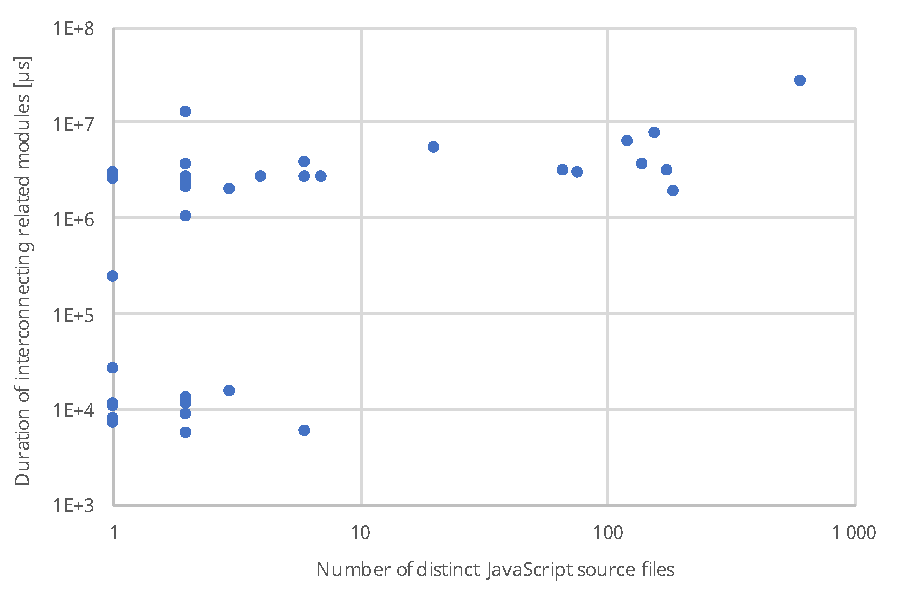
\includegraphics[width=\textwidth,clip]{figures/measurement-interconnecttime-modules.pdf}
	\caption{The characteristics of interconnecting related modules}
	\label{fig:measurement-interconnecttime-modules}
\end{figure}

\Cref{fig:measurement-interconnecttime-modules} shows the duration of interconnecting related modules in the light of the number of distinct modules in the repository. The figure shows that no relationship can be determined between the two values. Since the design of modularisation varies for every project, simply the number of distinct modules does not indicate how many of those modules are related to each other.


\subsection{The Qualifier System}

Spreading qualifiers along possible propagation paths in the Abstract Semantic Graph is a long process. In each propagation step, a particular qualifier can traverse only one relationship at a time — similarly to solving data-flow equations locally, based on the solution of the preceding equation. In larger graphs containing long transitive propagation paths, producing a full transitive closure can involve many steps.

The more \textquote{entry points} has a particular software for the Qualifier System (e.g.\ literals and \lstinline{throw} statements can be entry points: they get marked with a qualifier at the initialisation of the Qualifier System), the more propagation paths need to be closed up. The bigger the repository is, the more likely it is to contain such entry points.

\begin{figure}[!htb]
	\centerfloat
	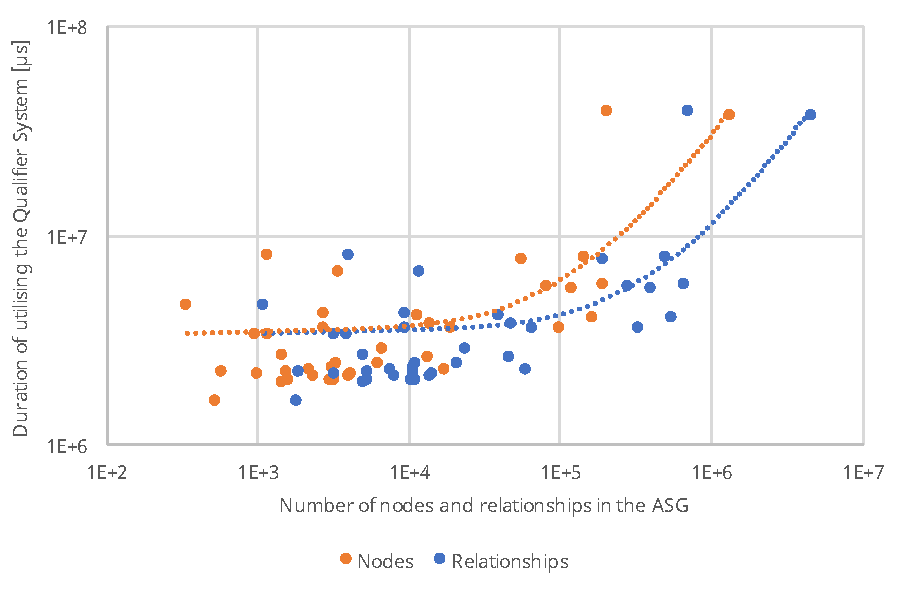
\includegraphics[width=\textwidth,clip]{figures/measurement-qualifiersystem-nodes-relationships.pdf}
	\caption{The characteristics of running the Qualifier System}
	\label{fig:measurement-qualifiersystem-nodes-relationships}
\end{figure}

\Cref{fig:measurement-qualifiersystem-nodes-relationships} presents the characteristics of the Qualifier System. The relationship between the duration of running the Qualifier System and the number of nodes and relationships in the ASG is not unequivocal, but an exponential trendline fits the dataset well. The Qualifier System's longest run took 38 seconds, at analysing the \lstinline{alvin198761/web-os} repository. For the \lstinline{tresorit/webclient}, the Qualifier System ran for 36 seconds. It is worth to mention here, that while the \lstinline{web-os} contains only 5,922 SLOC, the \lstinline{webclient} has 34,546. The similar duration of running the Qualifier System with this difference could imply that the \lstinline{web-os} contains much more defects to propagate qualifiers on.


\subsection{Analysis}

Importing, interconnecting, and applying the Qualifier System are only preparatory steps for running the actual analyses. All analyses involve matching complex patterns, even the ones using the results of the Qualifier System: besides qualifiers, several other attributes need to be queried for returning a complete set of analysis results, like code location information, and the containing module's file path.

\Cref{fig:measurement-analysis-nodes-relationships} presents the characteristics of the analyses. The duration of the analysis phase seemingly does not have any relationship with the number of graph nodes and relationships of a code repository. This is plausible, since the number of defects in a repository does not necessarily depends on the code base's size.

\vspace*{-2mm}
\begin{figure}[!htb]
	\centerfloat
	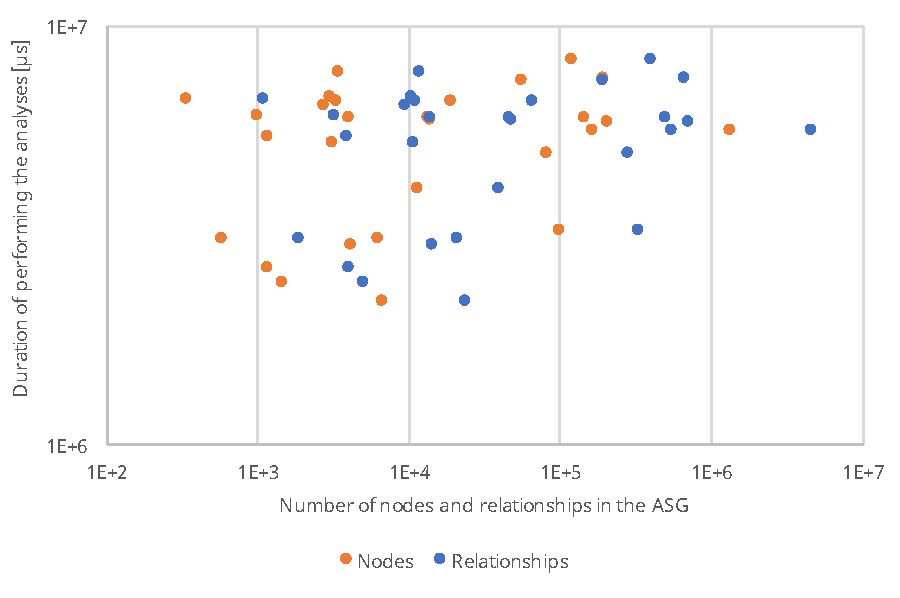
\includegraphics[width=\textwidth,clip]{figures/measurement-analysis-nodes-relationships.pdf}
	\caption{The characteristics of performing the analyses}
	\label{fig:measurement-analysis-nodes-relationships}
\end{figure}
\vspace*{-2mm}

\subsection{Total Duration of the Analysis Process}

The total duration of analysing a repository seems to be in linear relationship with the repository's size. \Cref{fig:measurement-totaltime-sloc} and \Cref{fig:measurement-totaltime-nodes-relationships} present that both measured in SLOC and in the number of graph nodes and relationships, there is a linear tendency: the bigger the source code repository, the more time it takes perform a complete analysis process on it.

It is interesting to notice by the detailed measurement data in the Appendix, that the proportion of the synchronisation phase's duration within the duration of the full analysis process increases with the size of the repository. While for the smaller repositories, the import makes up only 30–40\% of the total duration, for the larger repositories it increases to 80–90\%. For the \lstinline{tresorit/webclient} repository, the synchronisation phase makes up 98\% of the duration of the total analysis process.

\begin{figure}[!p]
	\centerfloat
	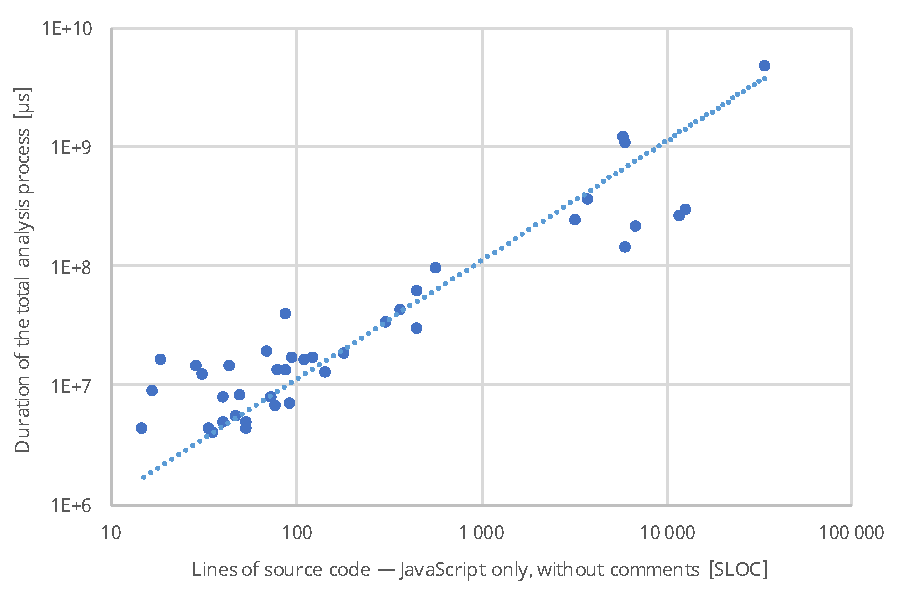
\includegraphics[width=\textwidth-1cm,clip]{figures/measurement-totaltime-sloc.pdf}
	\caption{The characteristics of the full analysis process}
	\label{fig:measurement-totaltime-sloc}
\end{figure}

\begin{figure}[!p]
	\centerfloat
	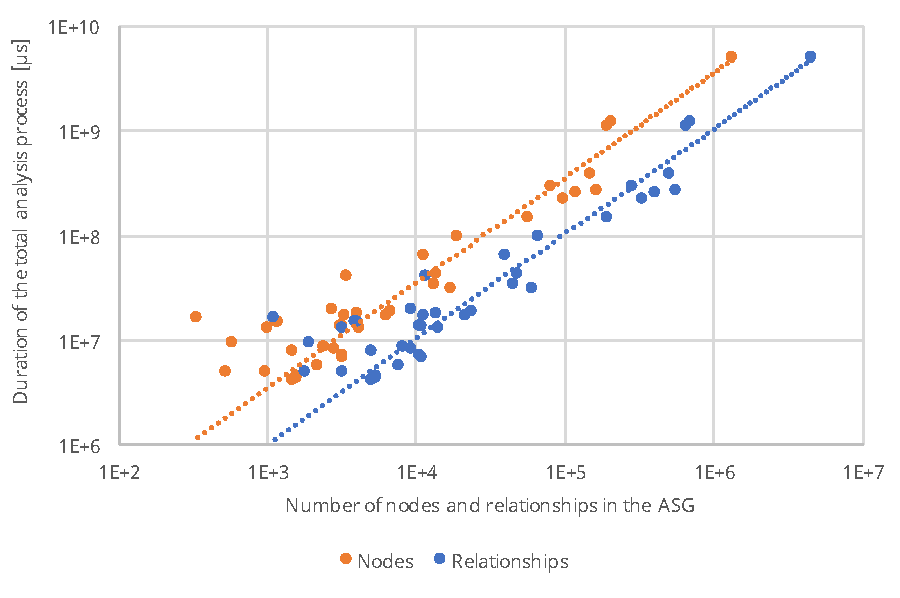
\includegraphics[width=\textwidth-1cm,clip]{figures/measurement-totaltime-nodes-relationships.pdf}
	\caption{The characteristics of the full analysis process}
	\label{fig:measurement-totaltime-nodes-relationships}
\end{figure}


\section{Defects Found by the Framework}

The framework found only two types of defects in the 40 analysed repositories: 897 cases of uninitialised variables, and 134 cases of globally unused exports were found. As the analysis is neither sound, nor complete, these numbers can be inaccurate. However, I inspected a randomly chosen subset of the found defects manually, and — according to my experience — the defects were indeed present in all cases.


\section{Threats to Validity}

I designed the measurements to be as accurate and complete as possible. Nevertheless, there are factors which I could not fully control, and these may have influenced the results. In this section, I summarise the factors which could bias the measurements.


\paragraph{Measurements on a Consumer Laptop}
Since my computer runs an operating system targeted for consumer usage, it may contain software running in the background, which influence measurement factors like processor or memory usage. I tried to mitigate these effects by configuring the computer to utilise all resources for the measurement procedure, by running the measurement processes multiple times, and by analysing a larger number of code repositories independently.


\paragraph{Graph Query Optimisations}
I tried to optimise the graph queries of the interconnections and the analyses as much as I could. However, since I am not an expert in the internals of Cypher queries, it is possible that some queries can be optimised further. Therefore, the characteristics of the interconnections or the analyses may not be fully correct.


\paragraph{Methological Mistakes}
It is possible that I made other methodological mistakes at implementing the analyses or the measurements. Using a fluid, internal semantics for the interconnection of modules incorrectly can be an example of a such mistake.